\chapter{Avaliação}
\label{cap:avaliacao}

%Durante as fases de análise e desenvolvimento existiu sempre a preocupação de efectuar uma análise funcional e de desempenho.



%\section{Ferramenta de testes e}
%Como efectuar a monitorização

%Foi desenvolvida uma aplicação para testar o desenvolvimento da ferramenta.
%Esta aplicação 

%\subsection{Test Unit}

%De forma a testar o repositório de dados foram efectuados diferentes \textit{unit tests}, de forma a assegurar que todas as alterações efectuadas na ferramenta ficavam de correctas.

%\subsection{Aplicação Monitora}
%\label{sub:monitor_app}

%Para poder mais facilmente efectuar os testes de avaliação, foi criado uma ferramenta em nível utilizador que permite lançar a aplicação e configurar automaticamente o sistema para a monitorizar. Esta verifica o identificador do processos e o momento em que se dá o inicio e o fim da sua execução, de forma a iniciar e terminar a monitorização quando necessário.

%\subsection{Aplicação de testes de performance}

%Para ajudar na avaliação da ferramenta desenvolvida foi criado um conjunto de aplicações independentes ( scripts e aplicações ) para monitorizar a actividade de algumas aplicações que se consideraram pertinentes no processo de avaliação do desempenho da ferramenta.

%A aplicação desenvolvida \textit{manager} tem de ser executada sob o controlo do utilizador \textit{root}, devido à necessidade de executar processos que só este utilizador tem acesso. Estes processos anteriormente mencionados são \textit{insmod}, \textit{rmmod} e \textit{tcpdump}.

%Os \textit{scripts} \textit{bash} criados serviram para obter o número de dados e pacotes transferidos na interface, bem como fazer a separação dos tempos que as aplicações de testes executaram para conseguir automatizar o processo de execução e recolha de dados dos testes.


%\section{Temporizadores}

%Temporizadores no núcleo do sistema.


%\subsection{Temporizadores de Alta-Resolução}

%\textit{HrTimer}


%----------------------------------------------------------------------------------------------------------

Antes de se implementar qualquer alteração, é conveniente proceder-se a testes alargados de verificação, para que se tome conhecimento do correcto funcionamento da aplicação e para que esta possa ser utilizada como uma mais–valia. 
O sistema implementado (MRoP) foi avaliado funcionalmente através da utilização de comandos para a transferência de dados baseados nos protocolos \textit{ftp}, \textit{http} e da aplicação \textit{iperf}\cite{iperf}.
Para o efeito recorreu-se a um conjunto alargado de testes, tendo como principal objectivo verificar o correcto funcionamento da aplicação, a capacidade de capturar todos os pacotes envolvidos nas comunicações do processo alvo (e apenas estes), bem como o seu desempenho e a sobrecarga introduzida.
A verificação da captura dos pacotes envolvidos nas comunicações do processo alvo foi feita através da ferramenta \textit{WireShark}, processo descrito na secção \ref{sec:eval_functional}.
Tendo em vista a realização de testes que avaliam o desempenho da aplicação, foram utilizadas duas máquinas, ligadas directamente, conforme o descrito  na secção \ref{sec:eval_performance}.
E por fim abordar-se-à detalhadamente o desempenho efectivo da aplicação.


\section{Avaliação Funcional}
\label{sec:eval_functional}


A análise funcional foi efectuada recorrendo a programas simples, que desencadeiam chamadas sucessivas de criação de sockets e comunicação, verificando-se o estado destes (portos e endereços) dentro do módulo do núcleo.
Estes dados foram confirmados no sistema de ficheiros \textit{DebugFs}, por consulta aos ficheiros existentes, para o efeito.
Este ficheiro quando acedido, contém toda a informação relativa aos portos e endereços em utilização, por parte da aplicação monitorizada.
Deste modo, para efectuar a comparação dos dados produzidos e validar esta análise, foi utilizada a ferramenta, \textit{netstat}, que indica os portos e endereços utilizados pelos processos no sistema.
A ferramenta anteriormente referida, utiliza o sistema de ficheiros virtual \textit{ProcFs}, para obter os dados dos portos e endereços, utilizados para comparação com os obtidos no MRoP.
Para além desta verificação, foi efectuada a confirmação de que todos os pacotes pertencentes às comunicações foram, de facto, correctamente obtidos.
Para tal, recorreu-se à captura de pacotes, por intermédio do \textit{tcpdump} com o módulo MRoP activo, constatando-se que todo o tráfego respeitante aos protocolos (\textit{ftp} e \textit{http}) estava de facto completo e correcto, desde a abertura ao fecho das conexões, não existindo outros pacotes na captura.
Esta validação foi efectuada utilizando o programa \textit{WireShark}, que identificou os fluxos de dados dos protocolos.


\section{Avaliação do desempenho}
\label{sec:eval_performance}

Tendo presente a avaliação do desempenho, foram efectuados diversos testes com o objectivo de avaliar a sobrecarga gerada pela introdução do \textit{MRoP}.
Estes testes basearam-se na recepção ou transmissão de 1 GigaByte de dados, utilizando diferentes programas e protocolos.
Ambas as máquinas, que se optou por designar de máquina 1 e máquina 2, procederam à transmissão/recepção de dados, utilizando cada uma apenas um processador activo, de 2 e 2.6 Ghz, respectivamente.
As máquinas anteriormente descritas encontravam-se conectadas directamente, por interfaces de rede a 100 MBit/s, ficando uma das máquinas responsável pela execução dos servidores \textit{ftp}, \textit{http} e \textit{iperf}, e a outra pelos respectivos clientes.
A versão do sistema de operação utilizado, em ambas as máquinas, correspondeu ao 2.6.39, sendo que na máquina 1 foram introduzidas algumas modificações para incluir o \textit{hook} do MRoP e as suas funções auxiliares, enquanto na máquina 2 se executou o sistema original, 2.6.39.

\subsection{Desempenho do MRoP}


Na execução destes testes, foram efectuadas 10 iterações, isto é, cada teste executado dez vezes, para cada experiência considerada, de modo a obter um valor médio e um desvio padrão considerado aceitável.
Os resultados obtidos constam das tabelas \ref{tab:desempenho} e \ref{tab:overhead}:

\begin{table}[!htb]
\begin{center}
\caption{Tempos médios em segundos (s)}
\begin{tabular}{ | c | c | c | c |  }
\hline
Teste & \hspace {0.3cm} Original \hspace {0.3cm}& \hspace {0.2cm} Com TcpDump \hspace {0.2cm} & Com TcpDump e MRoP \\
\hline
1GB - FTP$^{1}$ & 91.8508	& 91.8500 & 91.8854 \\
1GB - HTTP$^{2}$ & 91.6391 & 91.6472 & 91.6674 \\ 
IPerf - 1GB TCP$^{3}$ & 91.3790	& 91.2535	& 91.2672 \\
IPerf - 1GB UDP$^{4}$ & 89.7975 & 89.8007 & 89.8464 \\
\hline
\hline
1GB HTTP - 2 conexões$^{5}$ & 182.1573 & 188.7156 & 182.0161 \\
IPerf - 1GB UDP 2 conexões$^{6}$ & 179.4930 & 179.6280 & 179.6369 \\
\hline
\end{tabular}
\label{tab:desempenho}
\end{center}
\end{table}

\begin{table}[!htb]
\begin{center}
\caption{Sobrecarga das transferências (valores em percentagem)}
\begin{tabular}{ | c | c | c |}
\hline
Teste & \hspace {0.3cm} TcpDump \hspace {0.3cm} & TcpDump com MRoP  \\

\hline
1GB - FTP$^{1}$ & -0.0009  & 0.0377  \\
1GB - HTTP$^{2}$ & 0.0088 &  0.0309   \\
IPerf - 1GB TCP$^{3}$ & -0.1373 &  -0.1223   \\
IPerf - 1GB UDP$^{4}$ & 0.0036 & 0.0545 \\
\hline
\hline
1GB HTTP - 2 conexões$^{5}$ & 3.6003 & -0.0775   \\
IPerf - 1GB UDP 2 conexões$^{6}$ & 0.0752 & 0.0802   \\
\hline
\end{tabular}
\label{tab:overhead}
\end{center}
\end{table}

\begin{figure}[!ht]
\centering
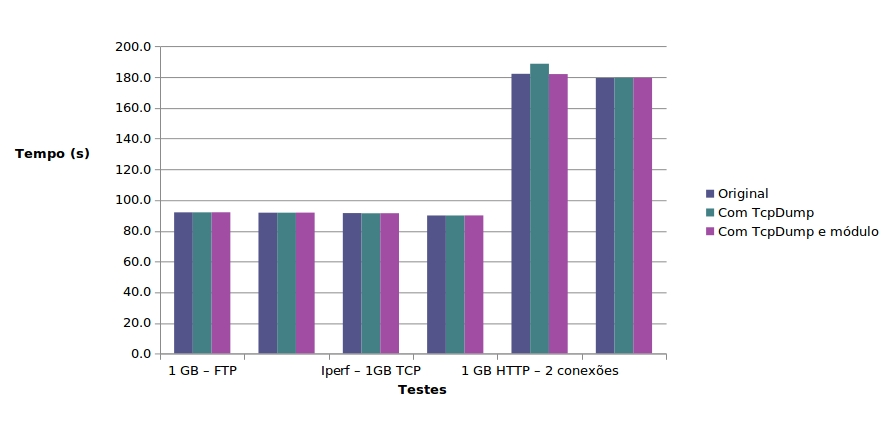
\includegraphics[scale=0.7]{testes.jpg}
\caption{Testes}
\label{fig:tests_graphics}
\end{figure}

\begin{figure}[!ht]
\centering
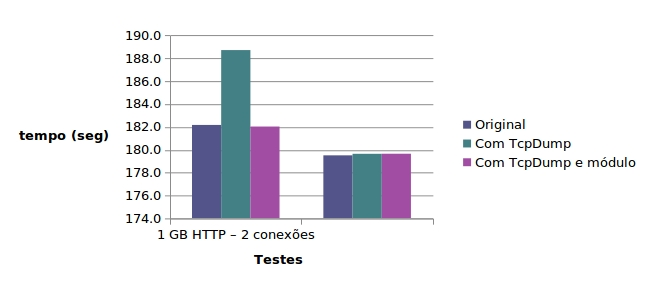
\includegraphics[scale=0.7]{overhead.jpg}
\caption{Sobrecarga nos testes 5 e 6 }
\label{fig:tests_overhead}
\end{figure}

Os testes identificados com os números de 1 a 4 foram efectuados utilizando apenas uma conexão ao servidor, enquanto os testes 5 e 6 foram efectuados utilizando mais uma comunicação, de modo a aumentar o peso sobre o processador e o número de pacotes a circular entre as máquinas.
Desta forma, foi possível identificar a sobrecarga exercida enquando o tcpdump estava a executar e a capturar todos os pacotes ou apenas um subconjunto destes, ou seja, os pertencentes aos processos alvo no novo sistema.
A coluna "Original" corresponde aos valores resultantes dos tempos médios das execuções das transferências sem qualquer monitorização.
A coluna "Com TcpDump" apresenta a média dos tempos de transferência com a captura total do tráfego, enquanto que a coluna identificada com "Com TcpDump e MRoP" regista a média dos tempos para a transferência com captura pelo tcpdump e o módulo MRoP desenvolvido no núcleo, de forma a capturar, apenas, o tráfego da transferência do processo alvo.
Nos primeiros quatro testes é possível verificar que a utilização do MRoP, aumentou de forma irrelevante o tempo de execução, Gráfico \ref{fig:tests_graphics}.
É igualmente possível observar que em 1 e 3, aquando da utilização do \textit{tcpdump}, a execução sem o MRoP, mostrou-se ligeiramente mais rápida, como se pode verificar na tabela \ref{tab:desempenho}.


Esta situação pode dever-se ao facto, de quando a máquina se encontra em sobrecarga, o sistema provoca o aumento do tamanho médio dos pacotes, reduzindo o seu número e o volume de dados transferidos, em virtude da diminuição dos seus cabeçalhos.

Nos testes 5 e 6, como o tráfego na interface é duplicado e o \textit{tcpdump} tem que capturar todos os pacotes, é possível evidenciar a sobrecarga exercida por estas cópias de dados e consequentes transferências, para nível utilizador face ao novo sistema que apenas captura um fluxo de dados.
Na tabela \ref{tab:overhead} e no gráfico tal tal é possível observar que, para o teste 5, a sobrecarga do \textit{tcpdump} atinge os 3.6\% face ao original, enquanto que a sobrecarga do \textit{tcpdump} com o MRoP, permitiu uma ligeira melhoria face ao original (-0.0775\%), como se pode observar no gráfico \ref{fig:tests_overhead}.
Conclui-se, portanto, que quando o fluxo de dados que não pretendemos capturar aumenta consideravelmente, torna-se mais vatajoso utilizar o MRoP, do que capturar todos os pacotes, na medida em que minimiza-se a sobrecarga, captura-se apenas os dados relevantes e evita-se a eventual análise em nível utilizador, para identificar e filtrar os pacotes pertencentes ao processo alvo, que acarreta ainda nova sobrecarga para além da aqui reportada.

\subsection{Desempenho da estrutura de dados}

Para além das avaliações anteriormente descritas, tornou-se essencial analisar o comportamento da estrutura de dados utilizada para manter o “estado do processo”, de modo a verificar o seu desempenho.
Assim, para esta análise, foi elaborado um teste que utiliza o sistema de alta resolução de temporizadores (HRTimer), contido no núcleo do sistema de operação. O teste consistiu em obter o tempo anterior e posterior à inserção dos 1024 elementos, afim de determinar o tempo decorrido.
De igual modo, foi calculado o tempo de remoção dos referidos elementos. Os resultados obtidos estão presentes na tabela \ref{tab:tree_info}.

\begin{table}[!htb]
\begin{center}
\caption{Custo das operações (tempos em nanosegundos)}
\begin{tabular}{ | r | c | c | }
\hline
\hspace{1cm} Teste \hspace{1.5cm} & \hspace{1cm}Duração\hspace{1cm} &  Média por
elemento \\
\hline
Adição de 1024 elementos & 869 244 & 848.8711 \\
\hline
Remoção de 1024 elementos & 675 086 & 659.2637\\
\hline

\hline
\end{tabular}
\label{tab:tree_info}
\end{center}
\end{table}

Como se pode verificar, pela tabela \ref{tab:tree_info}, a inserção de um elemento na árvore é inferior a 1 microsegundo, demonstrando que a estrutura utilizada foi a correcta.
Além de ter um bom compromisso de desempenho e utilização de memória, permitiu utilizar uma estrutura que já foi diversas vezes analisada, e a sua disponibilidade para utilização dentro do núcleo, permite ter um elevado grau de confiança na sua utilização.
O tempo médio despendido na procura do elemento com o menor valor de chave, nos 1024 elementos adicionados, foi de 1327 nanosegundos.
Com este valor é possível verificar que para efectuar 10 iterações de procura na árvore, incorre-se numa penalização de 1.3 microsegundos.
Verifica-se assim, que o tempo médio de procura de elementos na estrutura, neste caso, é menor ou igual a 1.3 microsegundos.
Considerando que a maior parte das aplicações não utiliza tantos portos em simultâneo, são expectáveis tempos inferiores em aplicações reais.


\subsection{Desempenho do Sistema de instrumentação}
Sendo a instrumentação das chamadas ao sistema um ponto fundamental na execução da monitorização de uma aplicação, a análise ao seu comportamento é bastante importante, na medida em que é necessário verificar se a introdução deste tipo de sistema irá produzir uma elevada penalização sobre o sistema de operação. A análise efectuada foi colocar um \textit{KRetProbe} na chamada ao sistema \textit{getpid} e avaliar o tempo decorrido entre o inicio e o fim do total das chamadas, com e sem o \textit{KRetProbe} de forma a avaliar a sobrecarga e verificar se coincide com o indicado pelos criadores do sistema.

\providecommand{\e}[1]{\ensuremath{\times 10^{#1}}}

\begin{table}[!htb]
\begin{center}
\caption{Duração das chamadas em segundos}
\begin{tabular}{ | c | c | c | c |}
\hline
Teste & Original & Com KretProbe & Sobrecarga por chamada\\
\hline
100 000 000 chamadas & 12.65 &  73.6600 & 610.10\e{-9}\\
1 000 000 000 chamadas & 126.85 & 737.2100 & 610.36\e{-9}\\
\hline
\end{tabular}
\label{tab:kprobes_info}
\end{center}
\end{table}

Os valores de referencia são de 0.7 microsegundos, os valores que foram obtidos foram de 0.61 microsegundos um pouco inferiores, pois a máquina de referência também tem velocidade inferior à máquina onde foram efectuados estes testes.

\section{Conclusão}
